\chapter{Introduction}
\hspace*{6mm}A surgical robot in assisting endodontic treatment -- DentiBot -- is presented in this thesis. DentiBot is designed to help dentists perform the root preparation procedure autonomously. This chapter will give brief introductions of the endodontic treatment, previous work, problem definition, and proposed method.
\section{Motivation}
\hspace*{6mm}Advancements in robot-assisted surgery invigorate the application of robotic technologies in dentistry. However, the majority of dental robot is applied in implantory. Research on robot-assisted Endodontic treatment is seldom explored. The performance of endodontic treatment depends on a dentist's long-term clinician experience and skill. A qualified dentist with a certification can operate an endodontic treatment. With enough clinical experience, the dentist can increase the success rate of surgery and acquire an endodontist license. According to statistics from the Ministry of Health and Welfare, R.O.C. (Taiwan) \cite{web1}, the number of dentists in Taiwan is $15,178$. However, according to The Academy of Endodontology, R.O.C. (Taiwan) \cite{web2}, only $238$ dentists own an endodontist license. It implies that performing an endodontic treatment requires the dentist's expertise of endodontics and enough clinical experience.  
\par
Besides, endodontic treatment is a tedious and time-consuming surgery for dentists due to intricate situations of toots. A patient who suffered from an infected tooth spends countless hours see a dentist. It might take two to three rounds of treatments, even more than two months in the worst case.  
\par
Therefore, our team looks forward to designing a robot-assisted system to accomplish endodontic treatment.  The robot-assisted system should have the capability to reduce times for entire treatment, increase the success rate of endodontic treatment for dentists, and provide patients a safer surgery.
\section{Problem Definition and Previous Work}
\hspace*{6mm}In this section, endodontic treatment is introduced followed by a brief description of related work and problem definition.
\subsubsection{Endodontic treatment}
\hspace*{6mm}Endodontic treatment, also known as root canal treatment and nerve extraction, is performed to cure an infected tooth. The main procedure of endodontic treatment is divided into three parts - Opening, Cleaning, and Filling shown in  Figure \ref{fig:endo-procedure}.
\par
An infected tooth arises from periodontal disease, attrition, trauma, or decay. Once the dental pulp is infected, it causes an irreversible inflammation and lets patients confront endodontic treatment. Figure \ref{fig:endo-procedure} shows an infected tooth and its dental pulp, which consists of blood vessels, nerves, connective tissues, and lymphatics. In the "Opening", a dentist drills the crown of the infected tooth to remove dentin and expose infected pulps inside canals to the air \cite{GUTMANN2011150}. Next,  "Cleaning" termed root preparation or debridement is the most essential step in entire endodontic treatment. Dentists uses an endodontic file, a superelastic root reamer, to remove the infected pulp thoroughly. It is necessary to ensure that there are no remained infected pulps \cite{GUTMANN2011195} after this procedure. Then, in the "Filling", the dentist uses a dental plugger to fill the empty root canal with Gutta-percha, a plastic substance. "Filling" can prevent cross-infection between root canals because the cured tooth remains many invisible and inaccessible pulp tissue \cite{GUTMANN2011218}. Finally, the dentist seals the root canal with a new crown to protect cured root canal and accomplishes endodontic treatment. 
\begin{figure}[htbp]
\begin{center}
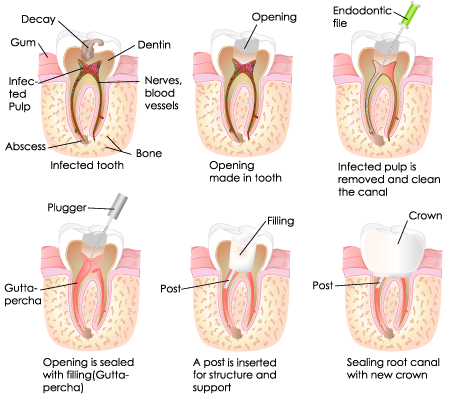
\includegraphics[width=0.75\linewidth]{Images/endo-procedure.png}
\caption[Endodontic treatment procedure]{Endodontic treatment procedure \cite{web7}}
\label{fig:endo-procedure}
\end{center}
\end{figure}
\par
As stated above, "Cleaning" is of paramount importance in whole treatment because cleaning improperly will result in pulp necrosis, apical abscess, periodontal ligament inflammation, or even cellulitis \cite{GUTMANN2011209}. If there are too many untreated contaminated canals, the treatment should be operated on again. Success in endodontic treatment depends on how well the dentist cleans and shapes the root canal. Therefore, it is important to figure out how a robot assists dentists in performing root canal treatment.
\subsubsection{Previous Work}
\hspace*{6mm}There are more and more robots which applied to specific surgery. In the dental field, the majority of robotic applications are in implant surgery. The researchers in Chosun University built a dental implant robot \cite{Kim2009ASO}, a remote center of motion (RCM) mechanism. Li, J. et al. designed a robotic system using a soft bracing technique to drill teeth \cite{Li2019ACD}. Also, there is a commercial implant robot, YOMI (Neocis ,Miami, FL). However, to the best of our knowledge there was one and only one robot for endodontic treatment. Janet Dong and his team proposed a microrobot performing endodontic treatment with a surgical path planned by 3-D root computer model \cite{dong2006wip}. However, the study using 3-D model belongs to pre-operation. Any patient moving or image error is a big challenge because it is not easy to reschedule the preoperative path because  root canals in a tooth are unseen by a camera from any angle. Besides, once an endodontic file enters into a root canal, it is hard to obtain the tool-tip of file due to its flexibility. The endodontic file will bend when it bears a force. Iatrogenic errors such as perforation, overpreparation, and underpreparation might happen. Therefore, a problem reveals -- how to adjust a surgical path to drill root canals in real-time and without visual feedback?
\par
On the other hand, instrument fracture is the other concern during endodontic treatment \cite{GUTMANN201197}. If an endodontic file suffers excessive usage, it would unpredictably break. The leading causes of fractured files are torsional fracture and flexural fatigue, which account for 55.7\% and 44.3\% separately \cite{SATTAPAN2000161}. Removal of a broken file in a small root is technically tricky, so it is essential to reduce the probability of the instrument fracture. Therefore, our robot should prevent the instrument fracture by some detection. In addition, endodontic treatment also requires repeatedly drilling to clean canals thoroughly. This repetitive action of root canal treatment is tedious and time-consuming. Therefore, It would be an efficient way to automate the root preparation procedure by an endodontic robot.
\subsubsection{Problem Definition}
\hspace*{6mm}To sum up, there are three main problems.
\begin{enumerate}
\item How to build an endodontic robot to assist dentists in performing the root preparation?
\item How to adjust the surgical path in real-time and without visual feedback in any intricate root situations?
\item How to protect the endodontic file from fracturing during the surgery?
\end{enumerate}	
\section{Proposed Method}
\hspace*{6mm}In this section, the prospect of DentiBot is presented followed by the proposed methods.
\subsubsection{Prospect}
\hspace*{6mm}To build a robot system for endodontic treatment, it is necessary to contemplate requirements and specifications comprehensively from technical and clinical perspectives. There are four subjects of the proposed robot-assisted project. 
\begin{enumerate}
	\item Dentist could move DentiBot to an infected tooth. 
	\item Searches all root canals of the infected tooth.
	\item Cleans roots thoroughly in the root preparation.
	\item Detects the apex of the root canal and accomplishes entire treatment.
\end{enumerate}	
\subsubsection{Design of DentiBot}
\hspace*{6mm}By comprehensive consideration, a robot-assisted system -- DentiBot -- is developed to provide a precise and safe endodontic treatment. DentiBot consists of a 6-DoF robot arm, a 1-DoF end effector modified from a dental handpiece, and a 6-DoF force/torque sensor. This 7-DoF robotic manipulator can manifest various motions such as drilling and reciprocation endodontic treatment requires. Therefor, DentiBot meets requirements of workspace and dimension in endodontic treatment.
\subsubsection{Force-Guided Robot Alignment}
\hspace*{6mm}Due to the lack of visual feedback in endodontic treatment, force-guided robot alignment based on admittance control techniques is proposed to guide the robot's motion. Force-guided alignment enables our system to adjust the surgical path and compensate for the patient's movement in real-time. That means DentiBot could align the root canal path by force feedback without vision feedback. Hence, force-guided alignment could solve the first failure factor -- incomplete root preparation.
\subsubsection{File Rotation and Feedrate Control}
\hspace*{6mm}To protect endodontic files from fracturing particularly when the file gets stuck in the root canal, two approaches based on  torque control are proposed. The first method, inverse rotation control, could remove debris and prevent files from getting stuck. The second method, file feedrate control, utilizes the measured file torque to regulate the file feedrate. These two proposed approaches are combined to protect endodontic files and achieve high performance in the root preparation procedure. 
\par 
A new idea that combines all proposed functions -- force guided alignment, inverse rotation control, and file feedrate control is presented.
\newpage
\section{Main Contributions}
\hspace*{6mm}In this section, main contributions of the thesis are highlighted followed by a brief description of the organization of the thesis.
\subsubsection{Main Contributions of the thesis}
\label{sec:contributions}
\hspace*{6mm}The thesis is the beginning of the proposed project and focuses on the first and  third subject of the project. In conclusion, there are three main contributions.
\begin{enumerate}
	\item	Integrate a 7-DoF robotic manipulator with 6-DoF F/T sensor for performing endodontic treatment.

	\item	Real-time Force-guided robot alignment for surgical path without visual feedback.
	\item	Inverse rotation control and File federate control for protecting the endodontic file from fracturing.
\end{enumerate}
\subsubsection{Organization of the Thesis}
\hspace*{6mm}In Chapter \ref{chapter2}, The state-of-the-art of dental robots for implant placement and endodontic treatment are surveyed and summarized. Implant robots including a commercial robot are reviewed and an endodontic robot is dissected. 
\par
The proposed robot -- DentiBot -- is highlighted in chapter \ref{chapter3}. Technical solutions to system integration with a robot arm are presented. The kinematics of the robot arm is derived. Moreover, how to find the tool-tip coordinate is explained.  
\par
Chapter \ref{chapter4} demonstrates how to solve the system integration problem when combining a robot arm and an F/T sensor. Gravity compensation and reference frame changing issues are clarified. Moreover, admittance control based on F/T sensor is presented. Subsequently, Force-guided robot alignment is described.  
\par
The proposed approach for protecting an endodontic file from fracturing is shown in Chapter \ref{chapter5}. File property is discussed and the methods for estimating torque are interpreted. Inverse rotation control and file feedrate control which are used to prevent instrument fracture are defined. Ultimately, the most important thing is that an algorithm for robot-assisted endodontic treatment is proposed.
\par
Experiment results are shown and analyzed in Chapter \ref{chapter6}. Technical and pre-clinical experiments are conducted. Force-guided alignment is confirmed by the first experiment and the proposed algorithm including all functions is proven by the second experiment.
In the end, Chapter \ref{chapter7} makes a summary and lists future work for this thesis.